% Copyright 2021 Joel Feldman, Andrew Rechnitzer and Elyse Yeager, except where noted.
% This work is licensed under a Creative Commons Attribution-NonCommercial-ShareAlike 4.0 International License.
% https://creativecommons.org/licenses/by-nc-sa/4.0/


 \begin{frame}{Table of Contents }
\mapofcontentsA{\ac,\aintro}
\label{note1.3a}
 \end{frame}
%----------------------------------------------------------------------------------------
\section{1.3: The Fundamental Theorem of Calculus}
%-------------------------------------------------------------
%----------------------------------------------------------------------------------------
\begin{frame}{Review: Area under a Curve}
\StatusBar{1}{10}
Methods for finding the area under a curve.\vfill
\begin{itemize}[<+->]
	\item Limit of a Riemann Sum
		\begin{itemize}[<+->]
			\item \textcolor{C1}{Conceptually} easy -- cut into rectangles\qquad \smash{\begin{tikzpicture} \clip (0,0) rectangle (2,1);
				\filldraw[fill=W5, fill opacity=0.5] (0,1) cos (2,0)-|(0,0);
				\filldraw[fill opacity=0.1] (0,0) rectangle (.5,1);
				\filldraw[fill opacity=0.1] (.5,0) rectangle (1,.8);
				\filldraw[fill opacity=0.1] (1,0) rectangle (1.5,.6);
				\filldraw[fill opacity=0.1] (1.5,0) rectangle (2,.2);
				\end{tikzpicture}}
			\item \textcolor{M3}{Computationally} rough \qquad \textcolor{gray}{$\lim\limits_{n \to \infty}\sum\limits_{i=1}^n f(x_i^*)\Delta x$;\quad $\sum\limits_{i=1}^n  i = \frac{n(n+1)}{2}$}
			\end{itemize}\vfill
	\item Use Geometry
			\begin{itemize}[<+->]
		\item \textcolor{M3}{Computationally} nice when it's available!\\
		 (Circles, triangles, symmetry, etc.)\qquad\qquad
		 \smash{\begin{tikzpicture} \clip (0,0) rectangle (2,1);
		 	\filldraw[fill=W5, fill opacity=0.5] (0,0) arc(180:0:1cm)--(0,0);
		 	\end{tikzpicture}}
		\item Often not available -- most functions\\
		 don't make such nice shapes.\qquad\qquad
		 \smash{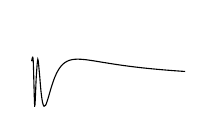
\begin{tikzpicture} \clip (0,0) rectangle (2,1);
		 	\draw plot[domain=.05:2, samples=100, smooth](\x,{.3*sin(1/\x r)+.3});
		 	\end{tikzpicture}}
	\end{itemize}\vfill
\item Up next: Fundamental Theorem of Calculus
		\begin{itemize}[<+->]
	\item \textcolor{C1}{Conceptually} less obvious -- we'll spend\\ about a day explaining \emph{why} it works
	\item \textcolor{M3}{Computationally} \emph{generally nicer} than Riemann sums
	\item Doesn't work for every function
\end{itemize}
	\end{itemize}
\end{frame}


%--------------------------------------------------------------------------------------------------------------------
%----------------------------------------------------------------------------------------
\newcommand{\FTCblock}{
	\begin{block}{Fundamental Theorem of Calculus, Part 1}
Let $a<b$ and let $f(x)$ be a function which is defined and continuous on $[a,b]$. Let
 \[A(x)=\int_a^x f(t)\,\dee t  \]
for any $x $ in $[a,b]$.
Then the function $A(x)$ is differentiable and

\[A'(x)=f(x)~.\]
\end{block}
\unote{Theorem~\eref{text}{thm:INTfundthmofcalc}}
	}
%----------------------------------------------------------------------------------------
\begin{frame}[t]
\FTCblock

\pause
\vfill
FTC(I) gives us the derivative of a very specific function (subject to some fine print).
\vfill
It shows a close relationship between integrals and derivatives.
\end{frame}
%
%%----------------------------------------------------------------------------------------


%----------------------------------------------------------------------------------------
\begin{frame}<1-8>[t]{Area Function: ${A(x)=\int_a^x f(t){\rm d} t \quad \text{ for } a \le x \le b }$}
\begin{center}
	\begin{tikzpicture}
	\myaxis{t}{0}{5}{y}{.0}{3}

 %show different values
\foreach \c in {2,...,8}{
	\DIVIDE{\c}{4}{\tempa}
	\ADD{\tempa}{2.5}{\tempb}
		\onslide<\c|handout:0>{	\xcoord{\tempb}{x}
		\fill[opacity=0.5, M4] plot[domain=1:\tempb, smooth](\x,{2- cos(\x r)})|-(1,0);
		}
	}
%show one value for printing
\onslide<handout>{
	\xcoord{4}{x}
	\fill[opacity=0.5, M4] plot[domain=1:4, smooth](\x,{2- cos(\x r)})|-(1,0);}

\draw[thick] plot[domain=0:5](\x,{2- cos(\x r)}) node[right]{$y=f(t)$};
\xcoord{1}{a}
	\end{tikzpicture}
	\end{center}
\onslide<4-|handout:2>{Notation: the function $A$ depends on the variable $x$.\medskip

We need to know how the function $f$ behaves on the whole interval $(0,x)$ to find $A(x)$. That's why we use $f(t)$, not $f(x)$.}
\StatusBar{2}{8}
\end{frame}
%----------------------------------------------------------------------------------------


\begin{frame}[t]{Area function notation}
\newcommand{\xx}{\textcolor{M4}{x}}
\newcommand{\xa}{\only<1-2>{\textcolor{M4}{1}}\only<3|handout:0>{\textcolor{M4}{2}}\only<4-|handout:0>{\textcolor{M4}{3}}}
\newcommand{\xb}{\only<5>{\textcolor{M4}{1}}\only<6|handout:0>{\textcolor{M4}{2}}\only<7-|handout:0>{\textcolor{M4}{3}}}
\newcommand{\xc}{\textcolor{M4}{1}}
\StatusBar{1}{8}
It might look strange at first to see two different variables. Let's consider the alternatives:


\begin{multicols}{3}
\noindent\begin{align*}
A(\xx)&=\int_0^{\xx} f(t)\,\dee t\\
\onslide<2->{A(\xa)&=\int_0^{\xa} f(t)\,\dee t}
\end{align*}

\begin{tikzpicture}
\myaxis{t}{0}{2}{y}{0}{2}
\draw[thick] plot[domain=0:2](\x,{sin(2*\x r)+1})node[above right]{$f(t)$};
\onslide<2>{\fill[M4, opacity=0.5] (0,0) --plot[domain=0:.5](\x,{sin(2*\x r)+1})|-cycle;\xcoord{.5}{\xa}}
\onslide<3|handout:0>{\fill[M4, opacity=0.5] (0,0) --plot[domain=0:1](\x,{sin(2*\x r)+1})|-cycle;\xcoord{1}{\xa}}
\onslide<4-|handout:0>{\fill[M4, opacity=0.5] (0,0) --plot[domain=0:1.5](\x,{sin(2*\x r)+1})|-cycle;\xcoord{1.5}{\xa}}
\end{tikzpicture}

\columnbreak

\noindent\begin{align*}
B(\xx)&=\int_0^{\xx} f(\xx)\,\dee t\\
\onslide<5->{B(\xb)&=\int_0^{\xb} f(\xb)\,\dee t}
\end{align*}
\onslide<5->{
\begin{tikzpicture}
\myaxis{t}{0}{2}{y}{0}{2}
\draw[help lines] plot[domain=0:2](\x,{sin(2*\x r)+1})node[above right]{$f(t)$};
\onslide<5|handout:0>{\draw[thick] (0,1.84)--(2,1.84);
\fill[M4, opacity=0.5] (0,0) rectangle (.5,1.84);
\ycoord{1.84}{f(\xb)} 
\xcoord{.5}{\xb}}
\onslide<6|handout:0>{\draw[thick] (0,1.91)--(2,1.91);
\fill[M4, opacity=0.5] (0,0) rectangle (1,1.91);
\ycoord{1.91}{f(\xb)} 
\xcoord{1}{\xb}}
\onslide<7-|handout:0>{\draw[thick] (0,1.14)--(2,1.14);
\fill[M4, opacity=0.5] (0,0) rectangle (1.5,1.14);
\ycoord{1.14}{f(\xb)}
\xcoord{1.5}{\xb}}
\end{tikzpicture}}

\columnbreak

\noindent\begin{align*}C(\xx)&=\int_0^{\xx} f(\xx)\,\dee \xx\\
\onslide<8->{C(\xc)&=\int_0^{\xc} f(\xc)\,\underbrace{\dee \xc}_{??}\\
}
\end{align*}



\end{multicols}
\end{frame}
%----------------------------------------------------------------------------------------
\begin{frame}[t]
\FTCblock

\pause
Question: Why is it true?
\end{frame}

%----------------------------------------------------------------------------------------

%----------------------------------------------------------------------------------------
\begin{frame}[t]{Derivative of Area Function, $A(x)=\int_a^x f(t){\rm d} t$}
\StatusBar{1}{8}
\begin{center}
	\begin{tikzpicture}[yscale=0.9]
	\myaxis{t}{0}{5}{y}{0}{3.1}
		\xcoord{3}{x} \xcoord{1}{a}
\onslide<-5|handout:1>{		\fill[opacity=0.5, M4] plot[domain=1:3, smooth](\x,{2- cos(\x r)})|-(1,0);}
\draw[thick] plot[domain=0:5](\x,{2- cos(\x r)}) node[right]{$y=f(t)$};
	\onslide<2-5|handout:1>{
		\draw[M4] (2,3.25) node{$A(x)$};}
	\onslide<3->{
		{\small \xcoord{4}{x+h}}
		}
\onslide<4-5|handout:1>{
	\fill[opacity=0.75,pattern color= C3, pattern=north east lines] plot[domain=1:4, smooth](\x,{2- cos(\x r)})|-(1,0);
	\draw[C3] (4,3.25) node{$A(x+h)$};}
\onslide<5-|handout:2>{
	\fill[opacity=0.75, C3] plot[domain=3:4, smooth](\x,{2- cos(\x r)})|-(3,0);
	\draw[M4, thick,dashed] (3,0) rectangle (4,3);}
\onslide<6-|handout:2>{	\draw[C3] (4,3.5) node{$A(x+h)-A(x)$};}
\onslide<7->{\ycoord{3}{f(x)}}

	\end{tikzpicture}
\end{center}

\small
$A'(x)=\lim\limits_{\Delta x \to 0}\frac{\Delta A}{\Delta x} = \lim\limits_{h \to 0}\frac{\only<-2|handout:0>{A(x+h)}\only<3->{\textcolor{C3}{A(x+h)}}-\alert<2-|handout:0>{A(x)}}{h}\onslide<7->{=\lim\limits_{h \to 0}\frac{\textcolor{C3}{hf(x)}}{h}}\onslide<8->{=f(x)}$\\[10pt]
\onslide<8-|handout:2>{\small When $h$ is very small, the purple area looks like a rectangle with base $h$ and height $f(x)$, so $\textcolor{C3}{A(x+h)-A(x) \approx hf(x)}$ and $\frac{A(x+h)-A(x)}{h}\approx f(x)$. As $h$ tends to zero, the error in this approximation approaches 0.}

\end{frame}

%----------------------------------------------------------------------------------------
\begin{frame}[t]
\QuestionBar<1>{1}{3}
\AnswerBar<2>{1}{3}
\sQuestionBar<3>{2}{3} \nsQuestionBar<2>{2}{3}
\AnswerBar<4>{2}{3}

\FTCblock

 Suppose $A(x)=\int_2^x \sin t\, \dee t$. What is $A'(x)$?\\[.5em]\pause
\sonslide{$A'(x)=\sin x$\pause}\vfill

 Suppose $B(x)=\int_x^2 \sin t\, \dee t$. What is $B'(x)$?\\[.5em]
\sonslide{ \pause $B'(x)=\diff{}{x}\left\{ -\int_2^x f(t)\,\dee t\right\}= -\sin x$ \vfill}
\vfill
\end{frame}

%----------------------------------------------------------------------------------------
\begin{frame}[t]
\QuestionBar<1>{3}{3}
\AnswerBar<2>{3}{3}


\FTCblock

Suppose $C(x)=\int_2^{e^x} \sin t\, \dee t$. What is $C'(x)$?\\[.5em]

\sonslide<2->{$C'(x)=e^x\sin (e^x)$: if we set $a=2$, then
\begin{align*}
C(x)&=A(e^x)\\
\implies C'(x)&=A'(e^x)\cdot\diff{}{x}\{e^x\}=\sin(e^x)\cdot e^x
\end{align*} }

\end{frame}

%----------------------------------------------------------------------------------------
%----------------------------------------------------------------------------------------
\begin{frame}[t]
\StatusBar{1}{6}
It's possible to have two different functions with the same derivative.
\begin{multicols}{2}\color{M4}
$A(x)=\int_0^x 2t\,\dee t$
\onslide<4->{$=x^2$}\\[7pt]
\begin{tikzpicture}
\myaxis{t}{0}{1.5}{y}{0}{1.5}
\draw[thick] (-.25,-.25)--(1.5,1.5);
\fill[pattern=north west lines,pattern color=M4](0,0)-|(1,1)--(0,0);
\xcoord{1}{x}
\end{tikzpicture}\\
\onslide<2->{$A'(x)=2x$}
\columnbreak\color{C3}

$B(x)=\int_1^x 2t\,\dee t$
\onslide<5->{$=x^2-1$}\\[7pt]
\begin{tikzpicture}
\myaxis{t}{0}{1.5}{y}{0}{1.5}
\draw[thick] (-.25,-.25)--(1.5,1.5);
\fill[pattern=north west lines,pattern color=C3](.5,0)-|(1,1)--(.5,.5)--cycle;
\xcoord{1}{x}
\xcoord{.5}{1}
\end{tikzpicture}\\
\onslide<3->{$B'(x)=2x$}
\end{multicols}\color{black}\normalsize
\onslide<6->{When two functions have the same derivative, \alert{they differ only by a constant}.\\[1em]

In this example: $B(x)=A(x)-1$}
\unote{Lemma~\eref{text}{lemma:+C}}
\end{frame}
%-------------------------------------------------------------
\begin{frame}[t]
\unote{Lemma~\eref{text}{lemma:+C}}
\begin{tikzpicture}[scale=0.9]
\myaxis{x}{0}{10}{y}{4}{3}
\foreach \y in {1,2,3,4,5}{
	\draw[C\y, thick] plot[domain=0:7,smooth](\x,{sin(\x r)+\y-3})node[right]{$f(x)+\y$};}
	\draw[black,thick] plot[domain=0:7,smooth](\x,{sin(\x r)-3})node[right]{$f(x)$};
\end{tikzpicture}\vfill
If two continuous functions have the same derivative, then one is a constant plus the other.
\end{frame}
%-------------------------------------------------------------
%----------------------------------------------------------------------------------------
\begin{frame}[t]
\only<2>{\QuestionBar{1}{3}}
\AnswerYes<2>
\AnswerBar<3>{1}{3}
Two clues for finding $A(x)=\int_a^x f(t) \, \dee t$:
\begin{itemize}
\item If $\displaystyle A(x)=\int_a^x f(t)\, \dee t$, then\footnote{(as long as $f(t)$ is continuous on $[a,x]$)}  $A'(x)=f(x)$
\item If $F'(x)=A'(x)$, then $A(x)=F(x)+C$ for some constant $C$.
\end{itemize}
\pause\vspace{1em}

$A(x)\displaystyle = \int_a^x e^t\, \dee t$. What functions could $A(x)$ be?\vfill
\sonslide<3->{
\begin{itemize}\color{spoilercolor}
\item $A'(x)=e^x$.
\item Guess a function with derivative $e^x$: $F(x)=e^x$.
\item Then $A(x)=e^x+C$ for some constant $C$.
\end{itemize}
}
\end{frame}
\addtocounter{footnote}{-1}
%----------------------------------------------------------------------------------------
%----------------------------------------------------------------------------------------
\begin{frame}[t]
\AnswerYes<1>\QuestionBar<1>{2}{3}
\AnswerBar<2>{2}{3}

Two clues for finding $A(x)=\int_a^x f(t) \, \dee t$:
\begin{itemize}
\item If $\displaystyle A(x)=\int_a^x f(t)\, \dee t$, then\footnote{(as long as $f(t)$ is continuous on $[a,x]$)}  $A'(x)=f(x)$
\item If $F'(x)=A'(x)$, then $A(x)=F(x)+C$ for some constant $C$.
\end{itemize}
\vspace{1em}

$A(x)\displaystyle = \int_a^x \cos t\, \dee t$. What functions could $A(x)$ be?\vfill
\sonslide<2->{
\begin{itemize}\color{spoilercolor}
\item $A'(x)=\cos x$.
\item Guess a function with derivative $\cos x$: $F(x)=\sin x$.
\item Then $A(x)=\sin x+C$ for some constant $C$.
\end{itemize}
}
\end{frame}
\addtocounter{footnote}{-1}
%----------------------------------------------------------------------------------------
%----------------------------------------------------------------------------------------
\begin{frame}[t]
\QuestionBar<1>{3}{3}
\AnswerYes<1>
\AnswerBar<2>{3}{3}

Two clues for finding $A(x)=\int_a^x f(t) \, \dee t$:
\begin{itemize}
\item If $\displaystyle A(x)=\int_a^x f(t)\, \dee t$, then\footnote{(as long as $f(t)$ is continuous on $[a,x]$)}   $A'(x)=f(x)$
\item If $F'(x)=A'(x)$, then $A(x)=F(x)+C$ for some constant $C$.
\end{itemize}
\vspace{1em}

$A(x)\displaystyle = \int_{-2}^x 5t^4\, \dee t$. What functions could $A(x)$ be?\vfill
\sonslide<2->{
\begin{itemize}\color{spoilercolor}
\item $A'(x)=5 x^4$.
\item Guess a function with derivative $5 x^4$: $F(x)=x^5$.
\item Then $A(x)= x^5+C$ for some constant $C$.
\item We ALSO know $A(-2)=\int_{-2}^{-2} 5t^4\, \dee t=0$, so we can find $C$:
\[0=A(-2)=(-2)^5+C \implies C=32\]
\item So, $A(x)=x^5+32$
\end{itemize}
}
\end{frame}
\addtocounter{footnote}{-1}
%----------------------------------------------------------------------------------------
%----------------------------------------------------------------------------------------
\begin{frame}[t]
\StatusBar{1}{6}\AnswerBar{3}{3}
\[A(x) = \int_{-2}^x 5t^4\, \dee t=x^5+32\]
\vfill
\begin{center}
\begin{tikzpicture}[yscale=0.9]
\onslide<+->{\myaxis{t}{4}{4}{y}{0}{4}
\draw[thick] plot[domain=-3.05:3.05, smooth](\x,{\x*\x*\x*\x/25})node[right]{$y=5t^4$};
\xcoord{-2}{-2}}

\foreach \b in {-1,...,3}{
	\onslide<+|handout:+>{
	\fill[C3,opacity=0.2] (-2,0)--plot[domain=-2:\b](\x,{\x*\x*\x*\x/25})|-cycle;
	\fill[pattern=north west lines, pattern color=C3] (-2,0)--plot[domain=-2:\b](\x,{\x*\x*\x*\x/25})|-cycle;
	\xcoord{\b}{\alert{\b}}
	\POWER{\b}{5}{\ax}
	\ADD{\ax}{32}{\Ax}
	\draw(0,-2)node{$\ds A(\alert{\b})=\int_{-2}^{\alert{\b}} 5t^4\, \dee t = (\alert{\b})^5+32=\Ax$};
	}}
	\end{tikzpicture}
	\end{center}

\end{frame}
%%----------------------------------------------------------------------------------------

%----------------------------------------------------------------------------------------
\newcommand{\xtob}{
	\only<-3|handout:1>{\alert<3|handout:0>{x}\vphantom{b}}\only<4-|handout:2>{\alert{b}}}
%----------------------------------------------------------------------------------------
\begin{frame}[t]
\StatusBar{1}{4}
\only<1>{\AnswerYes}
Two clues for finding $A(x)=\int_a^x f(t) \, \dee t$:
\begin{itemize}
\item If $\displaystyle A(x)=\int_a^x f(t)\, \dee t$, then\footnote{(as long as $f(t)$ is continuous on $[a,x]$)}  $A'(x)=f(x)$
\item If $F'(x)=A'(x)$, then $A(x)=F(x)+C$ for some constant $C$.
\end{itemize}
\vfill
$A(\xtob)\displaystyle = \int_a^{\xtob} f(t)\, \dee t$. What functions could $A(\xtob)$ be?\vfill
\onslide<2-|handout:2>{
\begin{itemize}
\item $A'(x)=f(x)$.
\item Guess a function with derivative $f(x)$: $F(x)$.
\item Then $A(x)=F(x)+C$ for some constant $C$.
\item Also $A(a)=0$, so $0=F(a)+C$, so $C=-F(a)$
\item So, $A(\xtob)=F(\xtob)-F(a)$
\end{itemize}
}
\end{frame}
\addtocounter{footnote}{-1}
%----------------------------------------------------------------------------------------
%----------------------------------------------------------------------------------------
\begin{frame}[t]
\StatusBar{1}{4}
\[\int_{a}^b f(t)\, \dee t=F(b)-F(a) \quad \text{where} \quad F'(x)=f(x)\]
\vfill
\begin{center}
\begin{tikzpicture}[yscale=0.9]
\onslide<+->{\myaxis{t}{3.5}{3.5}{y}{1}{3}
\draw[thick] plot[domain=-3.1:3.1, smooth,samples=50](\x,{\x*\x/3+sin(3*\x r)})node[right]{$y=f(t)$};
}

\foreach \a/\b in {-2/1,-2/2,-3/3}{
	\onslide<+|handout:+>{
	\fill[C3,opacity=0.2] (\a,0)--plot[domain=\a:\b,smooth](\x,{\x*\x/3+sin(3*\x r)})|-cycle;
	\fill[pattern=north west lines, pattern color=C3,smooth] (\a,0)--plot[domain=\a:\b](\x,{\x*\x/3+sin(3*\x r)})|-cycle;
	\xcoord{\b}{\b} \xcoord{\a}{\a}
	\POWER{\b}{5}{\ax}
	\ADD{\ax}{32}{\Ax}
	\draw(0,-2)node{$\ds \int_{\a}^{\b} f(t)\, \dee t = F(\b)-F(\a)$};
	}}
	\end{tikzpicture}
	\end{center}

\end{frame}
%%----------------------------------------------------------------------------------------
%----------------------------------------------------------------------------------------
%----------------------------------------------------------------------------------------
\begin{frame}[t]
\AnswerYes<2>\NoSpace<2>
\begin{block}{Fundamental Theorem of Calculus, Part 2}
Let $F(x)$ be differentiable, defined, and continuous on the interval $[a,b]$ with $F'(x)=f(x)$
for all $a<x<b$. Then
\[\int_a^b f(x)\,\dee{x} =F(b)-F(a) \]
\end{block}
\pause
Examples:\\
$\diff{}{x}\left\{5x^7 \right\}=35x^6$, so \\ $\ds\qquad\int_0^3 35x^6\,\dee x= $\sonslide<3->{
        $5x^7\Big|_{x=3}-5x^7\Big|_{x=0}=5(3^7)-5(0^7)=5\cdot3^7$  }\\ \vfill
$\diff{}{x}\left\{\tan x \right\}=\sec^2 x$, so \\ $\ds\qquad\int_0^{\pi/4} \sec^2 x\,\dee x= $\sonslide<4->{$ \tan x\Big|_{x=\frac{\pi}{4}}-\tan x\Big|_{x=0}=\tan(\pi/4)-\tan0=1$  }\vfill
\unote{Theorem~\eref{text}{thm:INTfundthmofcalc}}
\end{frame}
%----------------------------------------------------------------------------------------
\begin{frame}[t]
\[\int_{0}^3 35x^6\, \dee x=F(b)-F(a) \quad \text{where} \quad F(x)=5x^7\]
\vfill
\begin{center}
\begin{tikzpicture}
\myaxis{x}{1}{3.5}{y}{.5}{2}
\draw[thick] plot[domain=-1:3.1, smooth](\x,{\x^6/400})node[right]{$y=35x^6$};
\fill[C3,opacity=0.2] (0,0)--plot[domain=0:3](\x,{\x^6/400})|-cycle;
\fill[pattern=north west lines, pattern color=C3] (0,0)--plot[domain=0:3](\x,{\x^6/400})|-cycle;
\xcoord{3}{3}
\draw(0,-2)node{$\ds \int_{0}^{3} 35x^6\, \dee x = 5(3)^7-5(0)^7$};
\end{tikzpicture}
\end{center}

\end{frame}
%----------------------------------------------------------------------------------------
\begin{frame}[t]
\[\int_{0}^{\pi/4} \sec^2 x\ \dee x=F(b)-F(a) \quad \text{where} \quad F(x)=\tan x\]
\vfill
\begin{center}
\begin{tikzpicture}[yscale=0.9,xscale=3]
\myaxis{x}{0}{1.5}{y}{0}{4}
\draw[thick] plot[domain=0:1.05, smooth](\x,{sec(\x r)*sec(\x r)})node[right]{$y=\sec^2x$};
\fill[C3,opacity=0.2] (0,0)--plot[domain=0:1](\x,{sec(\x r)*sec(\x r)})|-cycle;
\fill[pattern=north west lines, pattern color=C3] (0,0)--plot[domain=0:1](\x,{sec(\x r)*sec(\x r)})|-cycle;
\xcoord{1}{1}
\draw(0,-1.75)node{$\ds \int_{0}^{\pi/4} \sec^2 x\ \dee x = \tan\left(\frac\pi4\right)-\tan0=1$};
\end{tikzpicture}
\end{center}

\end{frame}
%%----------------------------------------------------------------------------------------

%----------------------------------------------------------------------------------------
\begin{frame}[t]{Relevant Vocabulary}
\sQuestionBar<3>{1}{3} \AnswerYes<3,5,7>
\AnswerBar<4>{1}{3}
\sQuestionBar<5>{2}{3} 
\AnswerBar<6>{2}{3}
\sQuestionBar<7>{3}{3} 
\AnswerBar<8>{3}{3}

\nsQuestionBar<3>{1}{3}
\nsQuestionBar<4>{2}{3}
\nsQuestionBar<5>{3}{3}

\begin{block}{Definition}
If $F(x)$ is a function whose derivative is $f(x)$, we call $F(x)$ an \textbf{antiderivative} of $f(x)$.
\end{block}\pause\vfill
Examples:\\
The derivative of $x^2$ is $2x$, so:\\
$x^2$ is an \textbf{antiderivative} of $2x$.\\ \pause\vfill
When $x>0$, the derivative of $\log x $ is $\frac1x$, so:\\\pause
\sonslide{$\frac1x$ is an \textbf{antiderivative} of $\log x$.\\
\pause}
\vfill
For all $x$, the derivative of $\log |x| $ is $\frac1x$, so:\\
\sonslide{\pause $\frac1x$ is an \textbf{antiderivative} of $\log |x|$.\\ 
} \vfill\pause
An antiderivative of $\sin x$ is  \sonslide{\pause $-\cos x$, because $\diff{}{x}\left\{-\cos x\right\}=\sin x$.}
\end{frame}
%----------------------------------------------------------------------------------------
\begin{frame}[t]{Convenient Notation}
\QuestionBar<2>{1}{2}\AnswerYes<2,4>
\AnswerBar<3>{1}{2}
\sQuestionBar<4>{2}{2}
\AnswerBar<5>{2}{2}
\nsQuestionBar<3>{2}{2}
\iftoggle{spoiler}{\COPY{5}{\endslide}}{\COPY{3}{\endslide}}
\ADD{\endslide}{1}{\endslideb}

\begin{block}{Definition}
	\[f(x)\Big|_a^b = f(b)-f(a) \]
	The function $f(x)$ evaluated from $a$ to $b$
\end{block}\pause
\only<2-\endslide>{\vfill
Examples:\vfill
$ (5x+x^2) \Big|_1^2= \sonly{\pause(10+4)-(5+1)}$\pause\vfill
$\left. \frac{x^2}{x+2} \right|_{5}^{-1}=\sonly{\pause \frac{1}{1}-\frac{25}{7}}$\vfill}
\only<\endslideb->{\begin{block}{FTC Part 2, Abridged}
\[\int_a^b f(x)\,\dee x = F(x)\Big|_a^b\]
where $F(x)$ is an antiderivative of $f(x)$
\end{block}}
\end{frame}
%----------------------------------------------------------------------------------------
\begin{frame}[t]
\AnswerYes<1,3>
\QuestionBar<1>{1}{2}
\AnswerBar<2>{1}{2}
\sQuestionBar<3>{2}{2} \nsQuestionBar<2>{2}{2}
\AnswerBar<4>{2}{2}



\begin{block}{Definition}
The \textbf{indefinite integral} of a function $f(x)$:
\[\int f(x)\,\dee x \]
means the \textit{most general} antiderivative of $f(x)$.
\end{block}
\vfill
Examples:\\ \vfill
$\ds\int 2x\,\dee x= $  \sonly{\pause $ x^2+C$, \hspace{2cm} $C$ ``arbitrary constant."} \pause \vfill

$\ds\int \frac1x\,\dee x= \sonly{\pause \log|x|+C}$\\ \vfill
Remember: two functions with the same derivative differ by a constant, so we include the ``$+C$" for indefinite integrals.

\end{frame}
%----------------------------------------------------------------------------------------
\begin{frame}[t]{Definite vs Indefinite Integrals}
For each pair of properties below, decide which applies to \textbf{\color{C4}definite} integrals, and which to \textbf{\color{M4}indefinite} integrals.
\begin{center}
	\begin{tabular}{|l|c|}
		\hline
		No limits (or bounds) of integration, $\int f(x)\,\dee x$ & \iftoggle{spoiler}{\onslide<2->{\textcolor{M4}{indefinite}}}{~\hspace{2cm}~}\\
		Limits (or bounds) of integration, $\int_a^b f(x)\,\dee x$&\sonslide<3->{\textcolor{C4}{definite}}\\
		\hline
		Area under a curve &\sonslide<4->{\textcolor{C4}{definite}}\\
		Antiderivative&\sonslide<5->{\textcolor{M4}{indefinite}}\\
		\hline
		Number &\sonslide<6->{\textcolor{C4}{definite}}\\
		Function &\sonslide<7->{\textcolor{M4}{indefinite}}\\
		\hline
		\end{tabular}
	\end{center}
\end{frame}

%--------------------
\begin{frame}[t]{Antidifferentiation by Inspection}
\foreach \q[count=\n, evaluate=\a using int(\q+1)] in {1,3,...,15}{
	\nsQuestionBar<\n>{\n}{9}
	\sQuestionBar<\q>{\n}{9}\AnswerYes<\q>
	\AnswerBar<\a>{\n}{9}
	
	}


\begin{enumerate}[<+->]
\item $\displaystyle \int e^x\ \dee x$ \sonslide<+->{$=e^x+C$}
\item $\displaystyle \int \cos x\ \dee x$ \sonslide<+->{$=\sin x+C$}
\item $\displaystyle \int -\sin x\ \dee x$ \sonslide<+->{$=\cos x+C$}
\item $\displaystyle \int \frac1x\ \dee x$ \sonslide<+->{$=\log |x|+C$}
\item $\displaystyle \int 1\ \dee x$ \sonslide<+->{$=x+C$}
\item $\displaystyle \int 2x\ \dee x$ \sonslide<+->{$=x^2+C$}
\item $\displaystyle \int nx^{n-1}\ \dee x$ \sonslide<+->{$=x^{n}+C$} \qquad ($n\ne 0$, constant)
\item $\displaystyle \int x^{n}\ \dee x$ \sonslide<+->{$=\frac{1}{n+1}x^{n+1}+C$ } \qquad ( $n \neq -1$, constant)
\end{enumerate}

\end{frame}

%-------------------------------------------------------------
%----------------------------------------------------------------------------------------
%----------------------------------------------------------------------------------------
\begin{frame}[t]
\begin{block}{Power Rule for Antidifferentiation}
	\[\int x^n\, \dee x=\frac{1}{n+1}x^{n+1}+C \]
	if $n \neq -1$ is a constant
\end{block}
Example:\\
$\displaystyle\int \left(5x^2-15x+3 \right)\,\dee x=\sonly<2->{ \frac53x^3-\frac{15}{2}x^2+3x+C}$
\QuestionBar<1>{9}{9} \AnswerYes<1>
\AnswerBar<2>{9}{9}
\end{frame}

%----------------------------------------------------------------------------------------
\begin{frame}{Antiderivatives to Recognize}
\begin{itemize}
\item $\int x^n\ \dee x=\frac{1}{n+1}x^{n+1}+C$
\item  $\int a \ \dee x=ax+C$ 
\item $\int e^x\ \dee x=e^x+C$
\item	$\int\frac{1}{x}\ \dee x=\log|x|+C$ 
\item $\int \sin x \ \dee x=-\cos x +C$ 
\item $\int \cos x \ \dee x=\sin x +C$
\item	$\int \sec^2 x \ \dee x=\tan x +C$ 
\item $\int \sec x \tan x \ \dee x=\sec x +C$ 
\item $\int \csc x \cot x \ \dee x=-\csc x +C$
\item	$\int \csc^2 x \ \dee x=-\cot x +C$ 
\item $\int \frac{1}{1+x^2}\ \dee x=\arctan x +C$ 
\item $\int\frac{1}{\sqrt{1-x^2}} \ \dee x=\arcsin x +C$
\end{itemize}
\unote{Theorem~\eref{text}{thm imp indef int}}
\end{frame}
%----------------------------------------------------------------------------------------
%%----------------------------------------------------------------------------------------
%----------------------------------------------------------------------------------------
%----------------------------------------------------------------------------------------
%--------------------------------------------------------------------------------------------------------------------


